

\tikzset{every picture/.style={line width=0.75pt}} %set default line width to 0.75pt        

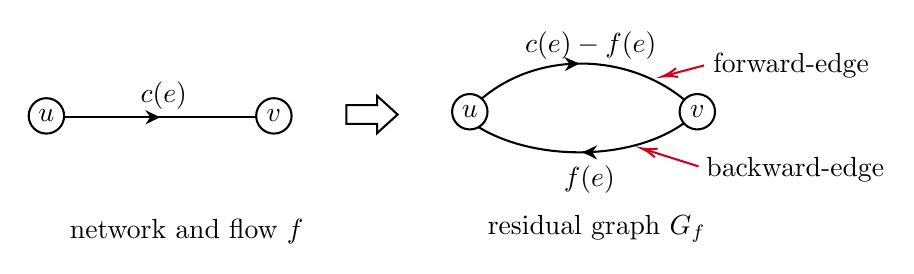
\begin{tikzpicture}[x=0.5pt,y=0.5pt,yscale=-1,xscale=1]
%uncomment if require: \path (0,177); %set diagram left start at 0, and has height of 177

%Curve Lines [id:da27260410535946566] 
\draw    (321,73) .. controls (363,22) and (445,23) .. (489.62,69.5) ;
\draw [shift={(404.33,34.69)}, rotate = 538.0899999999999] [fill={rgb, 255:red, 0; green, 0; blue, 0 }  ][line width=0.08]  [draw opacity=0] (10.72,-5.15) -- (0,0) -- (10.72,5.15) -- (7.12,0) -- cycle    ;
%Curve Lines [id:da29997342467331434] 
\draw    (321,73) .. controls (362,108) and (452,108) .. (489.62,69.5) ;
\draw [shift={(406.58,98.81)}, rotate = 0.2] [fill={rgb, 255:red, 0; green, 0; blue, 0 }  ][line width=0.08]  [draw opacity=0] (10.72,-5.15) -- (0,0) -- (10.72,5.15) -- (7.12,0) -- cycle    ;
%Straight Lines [id:da010972519675235493] 
\draw    (183.62,73.5) -- (19.22,73.5) ;
\draw [shift={(101.42,73.5)}, rotate = 180] [fill={rgb, 255:red, 0; green, 0; blue, 0 }  ][line width=0.08]  [draw opacity=0] (10.72,-5.15) -- (0,0) -- (10.72,5.15) -- (7.12,0) -- cycle    ;
%Shape: Ellipse [id:dp48830544834331435] 
\draw  [fill={rgb, 255:red, 255; green, 255; blue, 255 }  ,fill opacity=1 ] (6.43,72.5) .. controls (6.43,65.44) and (12.15,59.71) .. (19.22,59.71) .. controls (26.28,59.71) and (32.01,65.44) .. (32.01,72.5) .. controls (32.01,79.57) and (26.28,85.29) .. (19.22,85.29) .. controls (12.15,85.29) and (6.43,79.57) .. (6.43,72.5) -- cycle ;
%Shape: Ellipse [id:dp5269749982517756] 
\draw  [fill={rgb, 255:red, 255; green, 255; blue, 255 }  ,fill opacity=1 ] (170.83,72.5) .. controls (170.83,65.44) and (176.56,59.71) .. (183.62,59.71) .. controls (190.69,59.71) and (196.41,65.44) .. (196.41,72.5) .. controls (196.41,79.57) and (190.69,85.29) .. (183.62,85.29) .. controls (176.56,85.29) and (170.83,79.57) .. (170.83,72.5) -- cycle ;
%Shape: Ellipse [id:dp19207664116491352] 
\draw  [fill={rgb, 255:red, 255; green, 255; blue, 255 }  ,fill opacity=1 ] (312.43,69.5) .. controls (312.43,62.44) and (318.15,56.71) .. (325.22,56.71) .. controls (332.28,56.71) and (338.01,62.44) .. (338.01,69.5) .. controls (338.01,76.57) and (332.28,82.29) .. (325.22,82.29) .. controls (318.15,82.29) and (312.43,76.57) .. (312.43,69.5) -- cycle ;
%Shape: Ellipse [id:dp6327110520101094] 
\draw  [fill={rgb, 255:red, 255; green, 255; blue, 255 }  ,fill opacity=1 ] (476.83,69.5) .. controls (476.83,62.44) and (482.56,56.71) .. (489.62,56.71) .. controls (496.69,56.71) and (502.41,62.44) .. (502.41,69.5) .. controls (502.41,76.57) and (496.69,82.29) .. (489.62,82.29) .. controls (482.56,82.29) and (476.83,76.57) .. (476.83,69.5) -- cycle ;
%Right Arrow [id:dp9435587998338902] 
\draw   (236,64.75) -- (258.2,64.75) -- (258.2,58) -- (273,71.5) -- (258.2,85) -- (258.2,78.25) -- (236,78.25) -- cycle ;
%Straight Lines [id:da786288103209363] 
\draw [color={rgb, 255:red, 208; green, 2; blue, 27 }  ,draw opacity=1 ]   (494.5,36) -- (466.43,43.48) ;
\draw [shift={(464.5,44)}, rotate = 345.07] [color={rgb, 255:red, 208; green, 2; blue, 27 }  ,draw opacity=1 ][line width=0.75]    (10.93,-3.29) .. controls (6.95,-1.4) and (3.31,-0.3) .. (0,0) .. controls (3.31,0.3) and (6.95,1.4) .. (10.93,3.29)   ;
%Straight Lines [id:da5256035535625604] 
\draw [color={rgb, 255:red, 208; green, 2; blue, 27 }  ,draw opacity=1 ]   (490.5,109) -- (451.41,96.6) ;
\draw [shift={(449.5,96)}, rotate = 377.59000000000003] [color={rgb, 255:red, 208; green, 2; blue, 27 }  ,draw opacity=1 ][line width=0.75]    (10.93,-3.29) .. controls (6.95,-1.4) and (3.31,-0.3) .. (0,0) .. controls (3.31,0.3) and (6.95,1.4) .. (10.93,3.29)   ;

% Text Node
\draw (183.62,72.5) node   [align=left] {$\displaystyle v$};
% Text Node
\draw (19.22,72.5) node   [align=left] {$\displaystyle u$};
% Text Node
\draw (85,45.5) node [anchor=north west][inner sep=0.75pt]   [align=left] {$\displaystyle c( e)$};
% Text Node
\draw (489.62,69.5) node   [align=left] {$\displaystyle v$};
% Text Node
\draw (325.22,69.5) node   [align=left] {$\displaystyle u$};
% Text Node
\draw (363,9.5) node [anchor=north west][inner sep=0.75pt]   [align=left] {$\displaystyle c( e) -f( e)$};
% Text Node
\draw (391,106.5) node [anchor=north west][inner sep=0.75pt]   [align=left] {$\displaystyle f( e)$};
% Text Node
\draw (34,145) node [anchor=north west][inner sep=0.75pt]   [align=left] {network and flow $\displaystyle f$};
% Text Node
\draw (336,142) node [anchor=north west][inner sep=0.75pt]   [align=left] {residual graph $\displaystyle G_{f}$};
% Text Node
\draw (499,25) node [anchor=north west][inner sep=0.75pt]   [align=left] {forward-edge};
% Text Node
\draw (494,100) node [anchor=north west][inner sep=0.75pt]   [align=left] {backward-edge};


\end{tikzpicture}

